%%%%%%%%%%%%%%%%%%%%%%%%%%%%%%%%%%%%%%%%%%%%%%%%%%%%%%%%%%
\subsection{Cutoff Phenomenon}
%%%%%%%%%%%%%%%%%%%%%%%%%%%%%%%%%%%%%%%%%%%%%%%%%%%%%%%%%%
We also state the definition of a cutoff given by Diaconis in
\cite{Diaconis2005}. Assume that, to any finite set $\Omega$ and any
pair of probability measures $\omega$, $\bar{\omega}$ on $\Omega$ is associated
a real number $D(\omega,\bar{\omega})$ such that $D(\omega,\bar{\omega})\in [0,1]$,

\begin{eqnarray}
\max_{\Omega,\omega,\bar{\omega}} D(\omega,\bar{\omega}) = 1
\end{eqnarray}
and $D(\omega,\bar{\omega})=0$ if and only if $\bar{\omega}=\omega$. Consider a sequence of
(finite) probability spaces $(\Omega_n,\bar{\omega}_n)$, $n=1,2,...$, each
equipped with a sequence of probability measure $\omega^k_n$,
$l=0,1,...$, such that
\begin{eqnarray}
\lim_{k \rightarrow \infty} D(\omega_n,\bar{\omega}_n)=0
\end{eqnarray}
The definition of a cut-off is,

\begin{definition}
\label{cutoffdefinition}
(Diaconis) A family $(\Omega_n,\bar{\omega}_n, (\omega^k_n)_{k=0,1,...})_{n=1,2,...}$
presents a D-cut-off if there exists a sequence $(t_n)$ of positive
reals such that, for any $\epsilon \in(0,1)$,
\begin{enumerate}
  \item $\lim_{n \rightarrow \infty}D(\omega^{k_n}_n,\bar{\omega}_n) = 0 \mbox{ if }
  k_n>(1+\epsilon)t_n$
  \item $\lim_{n \rightarrow \infty}D(\omega^{k_n}_n,\bar{\omega}_n) = 1 \mbox{ if }
  k_n<(1-\epsilon)t_n $
\end{enumerate}
\end{definition}

In the next section, we need to relax the definition and set $\Omega_n$ to be infinite. We say that a family $(\Omega_n,\bar{\omega}_n, (\omega^k_n)_{k=0,1,...})_{n=1,2,...}$ presents a D-cut-off in the relaxed sense if it satisfies definition \ref{cutoffdefinition} but $\Omega_n$ is infinite. 


%%%%%%%%%%%%%%%%%%%%%%%%%%%%%%%%%%%%%%%%%%%%%%%%%%%%%%%%%%
\section{Cutoff Observed in 1-D Chaotic Map}
%%%%%%%%%%%%%%%%%%%%%%%%%%%%%%%%%%%%%%%%%%%%%%%%%%%%%%%%%%


Let $X = [0,1]$, on the measure space  $(X,\mathcal{A},\bar{\omega})$, for a given 1-D map $S: X \rightarrow X $ with $S(\bar{\omega})=\bar{\omega}$. The probability measure $\omega$  transported by $S$ in the following way, 
  \begin{eqnarray}
    \omega'(x')|dx'| = \omega(x)|dx|
  \end{eqnarray}
It is possible that there are more than one $x$ which give the same $x'$. Hence we actually have,
  \begin{eqnarray}
  \label{omegamap}
    \omega'(x') = \sum_i \left|\frac{dx_i}{dx'}\right|\omega(x) \mbox{   , for all } i \mbox{  such that  } x'=S(x_i)
  \end{eqnarray}
which is how the Perron-Frobenius operator works. In some cases we can write down the Perron-Frobenius operator explicitly, as we will see in some examples later. 


%%%%%%%%%%%%%%%%%%%%%%%%%%%%%%%%%%%%%%%%%%%%%%%%%%%%%%%%%%
\subsection{Tent Map Cutoff}
%%%%%%%%%%%%%%%%%%%%%%%%%%%%%%%%%%%%%%%%%%%%%%%%%%%%%%%%%%

\begin{figure}
\caption{\label{tentmapandlogisticmap} Tent Map and Logistic Map }
\centerline{\scalebox{0.5}[0.5]{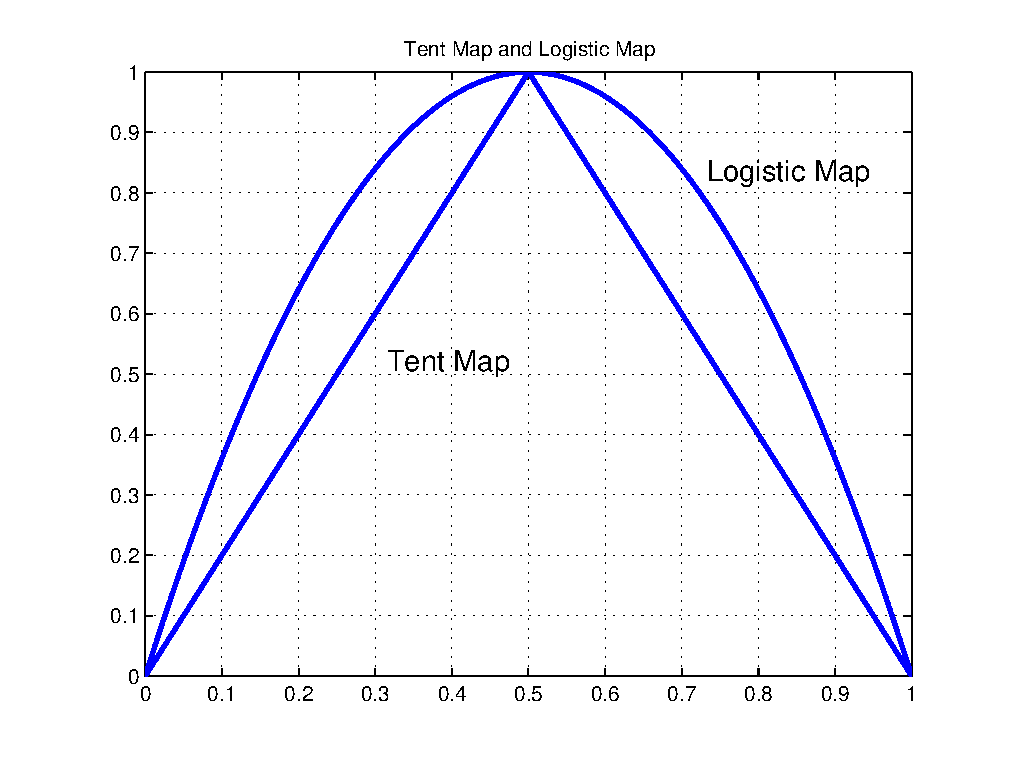
\includegraphics{tentmapandlogisticmap.eps}}}
\end{figure}


Consiter tent map,
   \begin{eqnarray}
   \label{tentmap}
     x' = S_\text{tent}(x) \equiv 1-2|x-\frac{1}{2}|
   \end{eqnarray}
with the following initial distribution on $[0 ,1]$
  \begin{eqnarray}
  \label{tentmapinitial}
    \omega_{\mu_n}^0 = \left\{ \begin{tabular}{c}
                      $\frac{1}{\mu_n}$, \mbox{  if  } $x \le \mu_n$\\ 
                      $0$, \mbox{  otherwise} 
                      \end{tabular}\right.
  \end{eqnarray}
where $\mu_1 = 1$, and $\mu_{k+1} = \frac{\mu_k}{2}$. By applying (\ref{omegamap}), the Perron-Frobenius operator of tent map is,
  \begin{eqnarray}
  \label{tentmapevolve}
    \omega_{\mu_n}^{k+1}(x) \equiv P_\text{tent} \omega_{\mu_n}^{k}(x)
                             = \frac{1}{2}\left( \omega_{\mu_n}^{k}\left(\frac{x}{2}\right)+
                                                 \omega_{\mu_n}^{k}\left(1-\frac{x}{2}\right)  \right)
  \end{eqnarray}
The invariant distribution $\bar{\omega}$ of tent map is uniform. Now consider the following sequence,
 \begin{eqnarray}
  \nu_{\mu_n}^k \equiv  |\omega_{\mu_n}^k-\bar{\omega} | 
 \end{eqnarray}
We have 
 \begin{eqnarray}
   \nu_{\mu_n}^k =  \left\{ \begin{tabular}{c} 
                    $1- 2^{1+k-n} $  ,if $k \le n-1$ \\
                    $0$   , otherwise
                    \end{tabular}\right.
 \end{eqnarray}
The of $\nu_{\mu_n}^k$ is in figure \ref{tentmapcutoff}. It clearly shows a cutoff. 

\begin{theorem} {\bfseries (Tent map cutoff)}

The family $([0,1],\bar{\omega}, (\omega^k_{\mu_n})_{k=0,1,...})_{n=1,2,...}$, where $\bar{\omega}$ is uniform in $[0,1]$ and $\omega^k_{\mu_n}$ are defined as in (\ref{tentmapinitial}) and (\ref{tentmapevolve}), presents a Total Variation-cut-off in the relaxed sense.
\end{theorem}




\begin{figure}
\caption{\label{tentmapcutoff} The plot of $\nu_{\mu_n}^k$}
\centerline{\scalebox{0.5}[0.5]{\includegraphics{tentmapcutoff.eps}}}
\end{figure}




%%%%%%%%%%%%%%%%%%%%%%%%%%%%%%%%%%%%%%%%%%%%%%%%%%%%%%%%%%
\subsection{Logistic Map Cutoff}
%%%%%%%%%%%%%%%%%%%%%%%%%%%%%%%%%%%%%%%%%%%%%%%%%%%%%%%%%%
Now let us turn to a more interesting case. Consider logistic map,  
  \begin{eqnarray}
  \label{logisticmap}
    S_\text{logistic}(x) = rx(1-x)
  \end{eqnarray}
with $r = 4$. Define initial distributions as
  \begin{eqnarray}
  \label{logisticmapinitial}
    \omega_{\mu_n}^0 = \left\{ \begin{tabular}{c}
                      $\frac{1}{\mu_n}$, \mbox{  if  } $x \le \mu_n$\\ 
                      $0$, \mbox{  otherwise} 
                      \end{tabular}\right.
  \end{eqnarray}
but now with  $\mu_0=1$, $\mu_{n+1}=\frac{1-\sqrt{1-\mu_n}}{2}$. This choice of $\omega_{\mu_n}^0$ is just to simplify the analysis and proof. Even if one chooses them as the ones we use in tent map, we would still observe cutoff. 

Again, by applying (\ref{omegamap}), we have
 \begin{eqnarray}
 \label{logisticmapevolve}
    \omega_{\mu_n}^{k+1}(x) &\equiv &P_\text{logistic} \omega_{\mu_n}^{k}(x)\\
                            &     = &\frac{1}{4\sqrt{1-x}}\left( \omega_{\mu_n}^{k}\left( \frac{1-\sqrt{1-x}}{2}\right)
                                            +\omega_{\mu_n}^{k}\left( \frac{1+\sqrt{1-x}}{2}\right) \right)
 \end{eqnarray}
The invariat distribution $\bar{\omega}$ for logistic map is 
\begin{eqnarray} 
\label{logisticmapinvariant}
 \bar{\omega} = \frac{1}{\pi\sqrt{x(1-x)}}
\end{eqnarray}
As before, we plot $\nu_{\mu_n}^k$ in figure \ref{logisticmapcutoff}.

\begin{figure}
\caption{\label{logisticmapcutoff} The plot of $\nu_{\mu_n}^k$}
\centerline{\scalebox{0.5}[0.5]{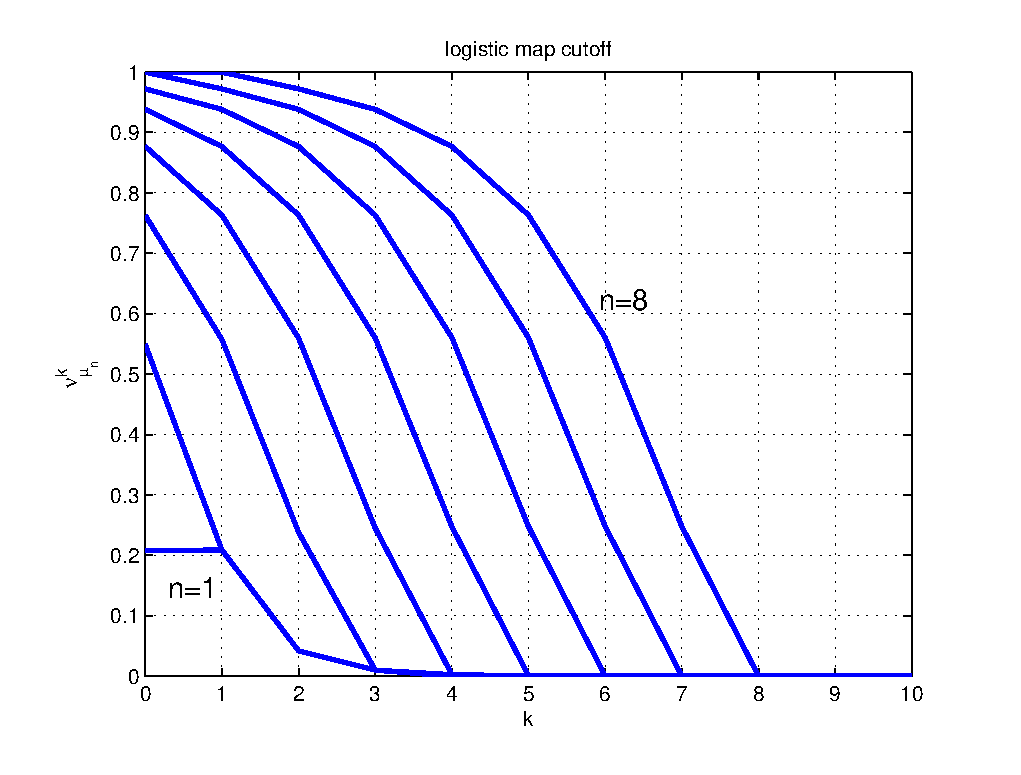
\includegraphics{logisticmapcutoff.eps}
                                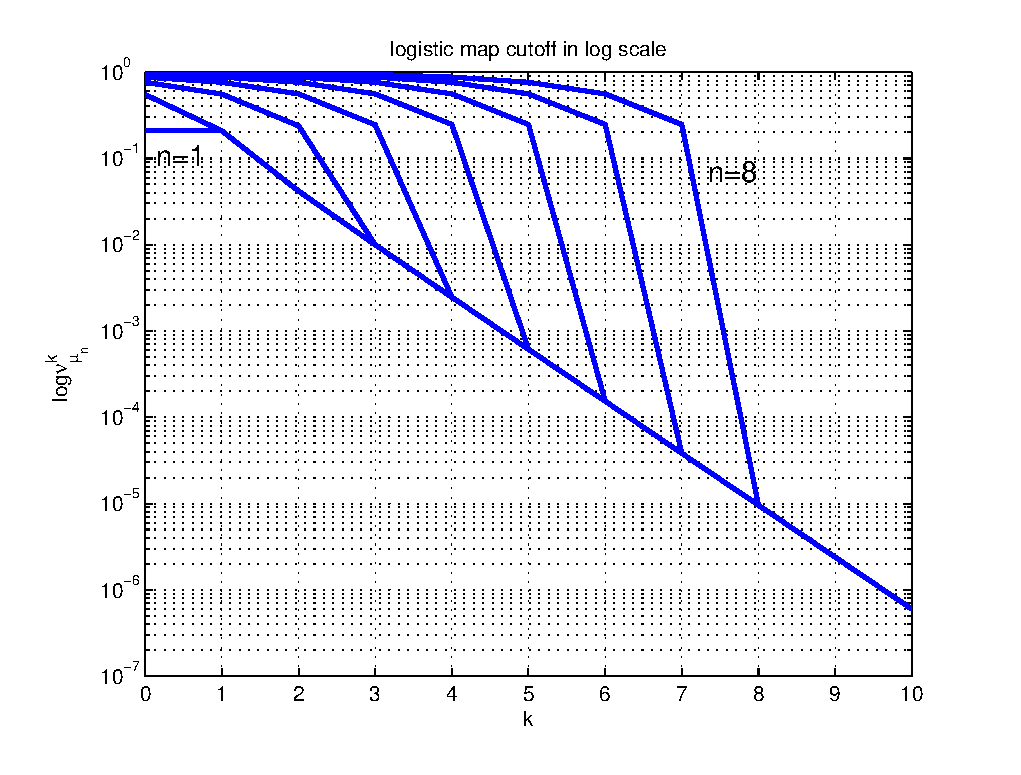
\includegraphics{logisticmapcutofflog.eps}}}
\end{figure}
The left plot in figure (\ref{logisticmapcutoff}) shows a similiar tendency as in (\ref{tentmapcutoff}). If we perform the simulation with more $n$s, the trajectories of $\nu_{\mu_n}^k$ will present a cutoff. In the log plot, one sees a more interesting thing: all the trajectories meet at some point and then decay exponentially with the same rate. 

It is well known that logistic map is equivalent to tent map by the follwoing transformation,
\begin{eqnarray} 
\label{tltransformation}
  x = \sin^2 \left(\frac{\pi y}{2}\right) \equiv T(y)
\end{eqnarray}
This means if $x$ and $y$ satisfy the above relation, then $S_\text{logistic}^k(x) = T(S_\text{tent}^k(y))$ for all $k \in \mathbb{N}$


We prove the following two lemmas.
%%%%%%%%%%%%%%%%%%%%%%%%%%%%%%%%%%%%%%%%%%%%%%%%%%%%%%%%%%
\begin{lemma}
\label{klenlemma}
When $k \ge 2$,
  \begin{eqnarray} 
     |\omega_{\mu_n}^k - \bar{\omega}|_{TV}>|\omega_{\mu_{n-1}}^{k-1} - \bar{\omega}|_{TV}
  \end{eqnarray}
for all $k \le n$ .
\end{lemma}
\paragraph{Proof} See appendix.


%%%%%%%%%%%%%%%%%%%%%%%%%%%%%%%%%%%%%%%%%%%%%%%%%%%%%%%%%%
\begin{lemma}
\label{kgenlemma}
When $n \ge 2$,
  \begin{eqnarray}
     \omega_{\mu_n}^k = \omega_{\mu_n-1}^{k}
  \end{eqnarray}
for all $k$ when $k \ge n$.
\end{lemma}
\paragraph{Proof} See appendix.



%%%%%%%%%%%%%%%%%%%%%%%%%%%%%%%%%%%%%%%%%%%%%%%%%%%%%%%%%%%
Now we have the following theorem
\begin{theorem} {\bfseries (Logistic map cutoff)}

The family $([0,1],\bar{\omega}, (\omega^k_{\mu_n})_{k=0,1,...})_{n=1,2,...}$, where $\bar{\omega}$ is defined as in (\ref{logisticmapinvariant}) and $\omega^k_{\mu_n}$ are defined as in (\ref{logisticmapinitial}) and (\ref{logisticmapevolve}), presents a Total Variation-cut-off between $k=n-1$ and $n$ in the relaxed sense .
\end{theorem}

\paragraph{Proof}
Total variation distance is non-increasing. By applying lemma \ref{klenlemma} and \ref{kgenlemma}, we obatin the theorem. 



  
%%%%%%%%%%%%%%%%%%%%%%%%%%%%%%%%%%%%%%%%%%%%%%%%%%%%%%%%%%
\subsection{Another map: $S= \sin(\pi x)$}
%%%%%%%%%%%%%%%%%%%%%%%%%%%%%%%%%%%%%%%%%%%%%%%%%%%%%%%%%%
One may suspect that lemma 2 holds for all chaotic maps similar to logistic map, but this is not true. Let us consider the following map,
 \begin{eqnarray}
    x' = \sin(\pi x)
 \end{eqnarray}
with $\mu_{n+1} = \frac{1}{\pi}\sin^{-1}(\mu_{n})$, and again $\omega_{\mu_n}^0$ is uniformly distributed in $[0, \mu_n]$ with value $\frac{1}{\mu_n}$. Figure \ref{halfsinmapcutoff} shows the $\nu_{mu_n}^k$ versus $k$ plots in normal and log scales. Clearly we do not observe the $\nu_{\mu_n}^k = \nu_{\mu_{n-1}}^{k}$ for $k \ge n$ hence lemma 2 cannot be true. However, still each trajectory shows a super-exponential decay region followed by an exponential decay region, and they presents a cutoff. In fact, we believe that cutoff happens for all chaotic map of this kind, but to prove it is not easy for most cases.  

\begin{figure}
\caption{\label{halfsinmapcutoff} The plot of $\nu_{\mu_n}^k$}
\centerline{\scalebox{0.5}[0.5]{\includegraphics{halfsinmapcutoff.eps}
                                \includegraphics{halfsinmapcutofflog.eps}}}
\end{figure}





%%%%%%%%%%%%%%%%%%%%%%%%%%%%%%%%%%%%%%%%%%%%%%%%%%%%%%%%%%
%%%%%%%%%%%%%%%%%%%%%%%%%%%%%%%%%%%%%%%%%%%%%%%%%%%%%%%%%%
\section{The Cutoff Observed in Advection-Diffusion Simulation}
%%%%%%%%%%%%%%%%%%%%%%%%%%%%%%%%%%%%%%%%%%%%%%%%%%%%%%%%%%
In the above studies, we use the same map and a sequence of different initial distributions to obtain the cutoff trajectories. Now we want to extend the study of cutoff phenomenon to another sequence of simulations. In this case we study the chaotic map with small diffusion. The sequence of convergence trajectoreis will be generated by a sequence of advection-diffusion operators. 




 
%%%%%%%%%%%%%%%%%%%%%%%%%%%%%%%%%%%%%%%%%%%%%%%%%%%%%%%%%%
\subsection{Cutoff in $\omega_n^k$}
%%%%%%%%%%%%%%%%%%%%%%%%%%%%%%%%%%%%%%%%%%%%%%%%%%%%%%%%%%
Consider standard map,

  \begin{eqnarray}
               x_1' &=& x_1+x_2 +\epsilon \sin{2 \pi x_1} (\mbox{ mod } 1) \nonumber\\
               x_2' &=&  x_2 +\epsilon \sin{2 \pi x_1}     (\mbox{ mod } 1)
  \end{eqnarray}

Now similar to the 1-D map case, we choose vector $\omega_n^0 = [1,0,0,...,0] \in \mathbb{R}^{n^2} $ to be the initial distribution, and evolve the Markov chain by $\omega_n^{k+1} = A^T \omega_n^{k}$. For $n = 1000$ the figure \ref{demostandardmapsing} shows some of the iterations.
\begin{figure} 
\caption{\label{demostandardmapsing}}
\centerline{\scalebox{0.6}[0.6]{
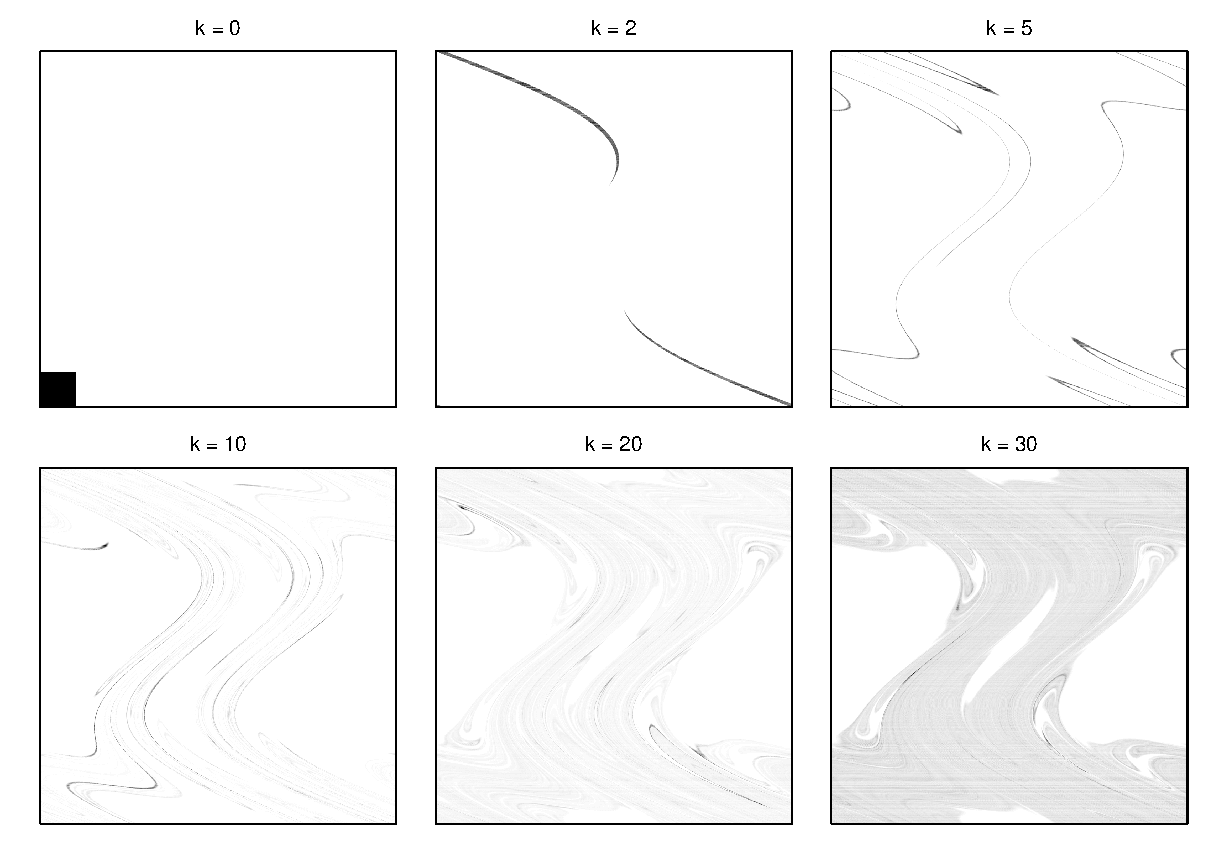
\includegraphics{demostandardmapsing.eps}
 }
}
\end{figure}
And then the cutoff figures (later)
  

%%%%%%%%%%%%%%%%%%%%%%%%%%%%%%%%%%%%%%%%%%%%%%%%%%%%%%%%%%
\subsection{Cutoff with initial condition $cos(2\pi x_2)$}
%%%%%%%%%%%%%%%%%%%%%%%%%%%%%%%%%%%%%%%%%%%%%%%%%%%%%%%%%%
The more interesting thing is that to choose $\omega_n^0 = [1,0,0,...,0]$ is not necessary for cutoff to happen. We use the following initial condition,
\begin{eqnarray}
  f_n^0 = g_n(\cos(2 \pi x_2))
\end{eqnarray}
And perform the iteration as $f_n^{k+1}= A_n f_n^k$. Selected iterations are plotted in figure \ref{demostandardmapcos}, and the trajectories of $\nu^k_n \equiv \sum_n |f^k-1|$ are shown in figure \ref{standardmapcutofftrajectory}. 

    
\begin{figure}
\caption{\label{demostandardmapcos}}
\centerline{\scalebox{0.6}[0.6]{
\includegraphics{demostandardmapcos.eps}
}}
\end{figure}


\begin{figure}
\caption{\label{standardmapcutofftrajectory}}
\centerline{
\begin{tabular}{rl}
\scalebox{0.4}[0.4]{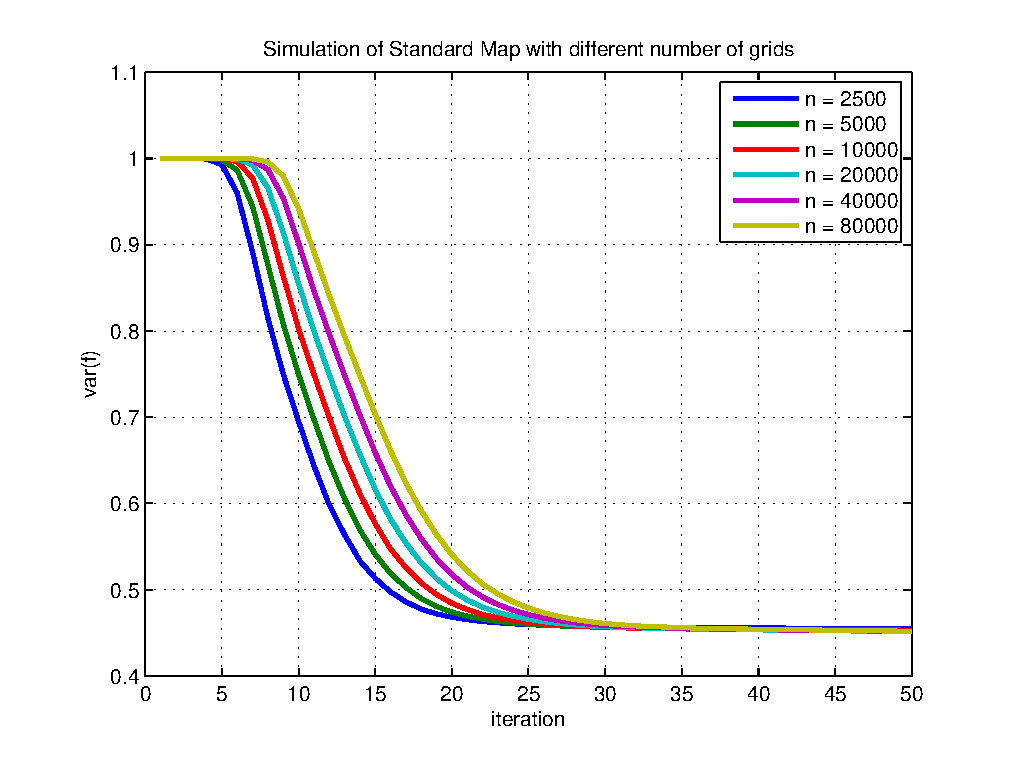
\includegraphics{standardmapcutoff}}&
\scalebox{0.4}[0.4]{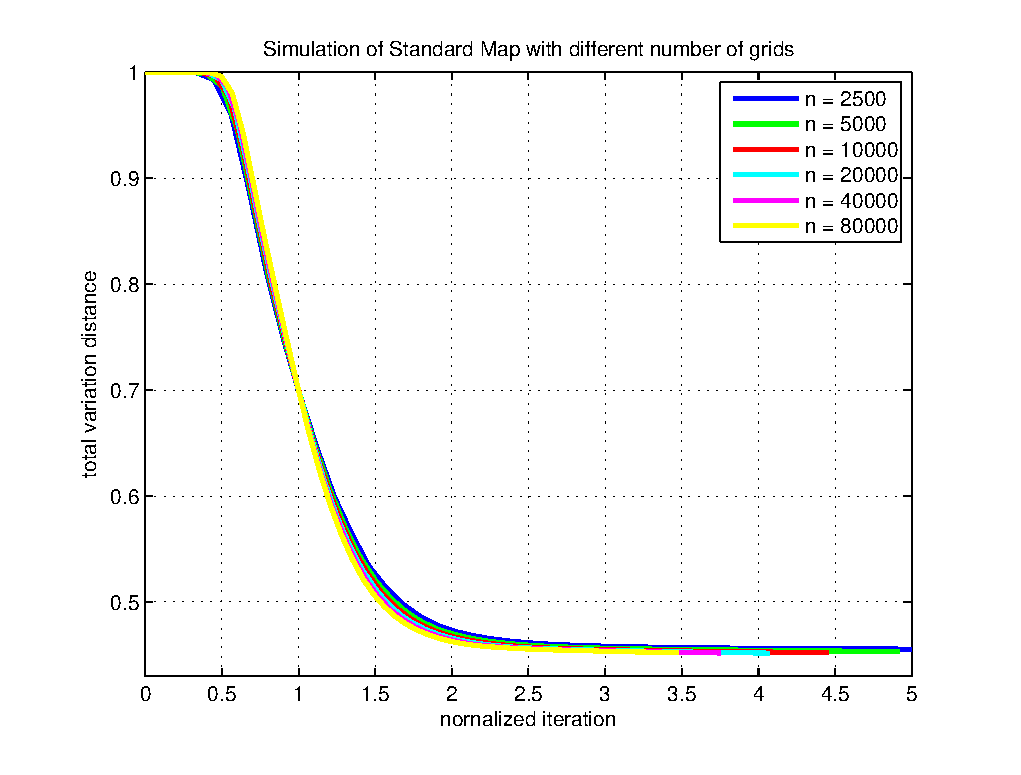
\includegraphics{standardmapcutoffn}}\\
\scalebox{0.4}[0.4]{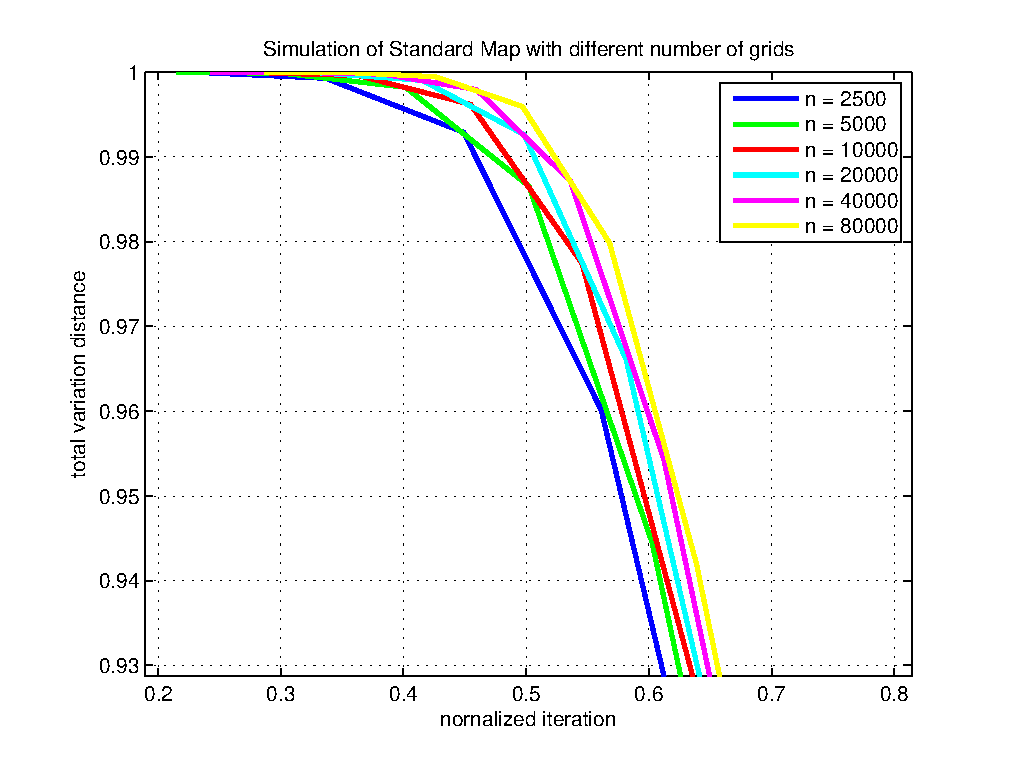
\includegraphics{standardmapcutoffmacro}}&
\scalebox{0.4}[0.4]{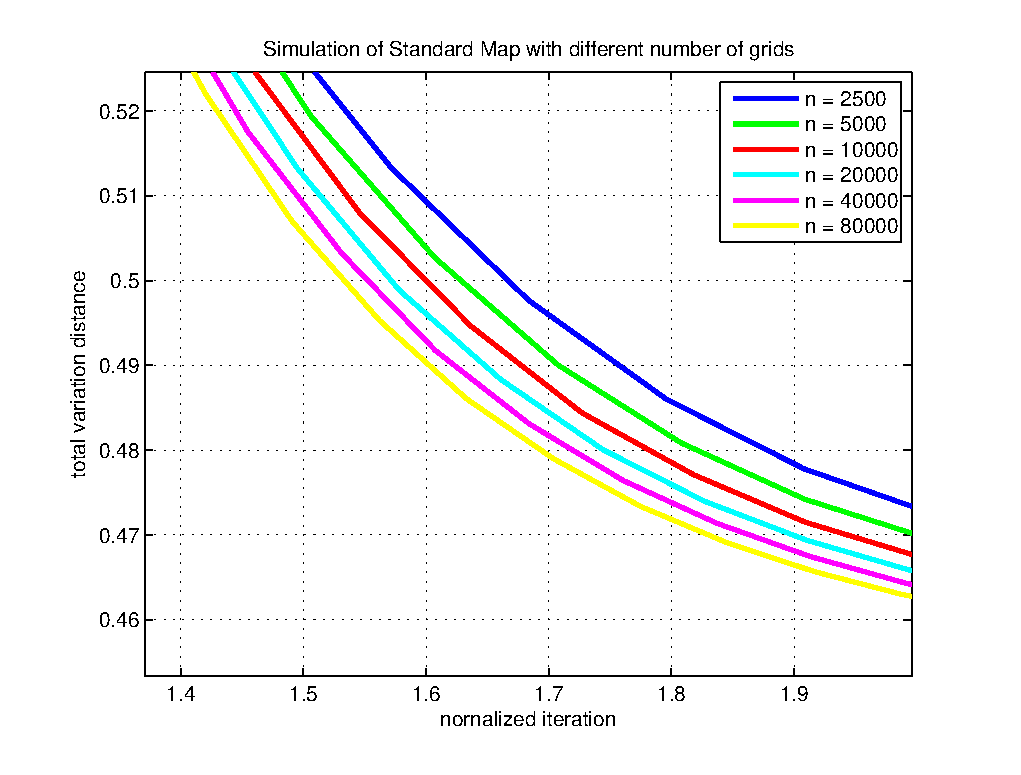
\includegraphics{standardmapcutoffmacro2}}
\end{tabular}
}
\end{figure}



%%%%%%%%%%%%%%%%%%%%%%%%%%%%%%%%%%%%%%%%%%%%%%%%%%%%%%%%%%
%%%%%%%%%%%%%%%%%%%%%%%%%%%%%%%%%%%%%%%%%%%%%%%%%%%%%%%%%%
\section{Appendix}
Here are the small lemmas I need.

proof of lemma \ref{klenlemma}
\paragraph{Proof}
Let $p_{\mu_n}^k$ be the point such that $\omega_{\mu_n}^k(p_{\mu_n}^k) = \bar{\omega}(p_{\mu_n}^k)$. By lemmas, we have  $p_{\mu_n}^k < p_{\mu_{n-1}}^{k-1}$, and $\omega_{\mu_n}^k(x)< \omega_{\mu_{n-1}}^{k-1}(x)$ for $x< p_{\mu_n}^k $, Let
 \begin{eqnarray}
  \Delta =  \int_0^{p_{\mu_{n-1}}^{k-1}} \omega_{\mu_{n-1}}^{k-1}(x) -\omega_{\mu_n}^k(x) dx
            +\int_{p_{\mu_{n-1}}^{k-1}}^{p_{\mu_n}^k} \bar{\omega}(x) - \omega_{\mu_n}^k(x) dx >0
 \end{eqnarray} 
 \begin{eqnarray}
    |\omega_{\mu_n}^k - \bar{\omega}|_{TV} 
                & = & \int_{S^k(\mu_n)}^1  \bar{\omega}(x) dx +
                      \int_0^{p_{\mu_n}^k} \bar{\omega}(x) - \omega_{\mu_n}^k(x)dx \nonumber\\  
                & = & \int_{S^{k-1}(\mu_{n-1})}^1  \bar{\omega}(x) dx +
                      \int_0^{p_{\mu_{n-1}}^{k-1}} \bar{\omega}(x) - \omega_{\mu_n}^k(x)dx + \Delta \nonumber\\
                & > & |\omega_{\mu_n-1}^{k-1} - \bar{\omega}|_{TV}
 \end{eqnarray}

proof of lemma \ref{kgenlemma}

\paragraph{Proof}
It suffices to prove $f(x)+ f(1-x) = 0$, where 
  \begin{eqnarray}
     f(x) \equiv \omega_{\mu_n}^{n-1}(x) -\omega_{\mu_n-1}^{n-1}(x)
  \end{eqnarray}
We will prove it by applying the transformation (\ref{tltransformation}). Let $\hat{\mu}_n = T^{-1}(\mu_n)$, and 
 \begin{eqnarray}
    \hat{\omega}_{\hat{\mu}_n^0}(y) = \left|\frac{dx}{dy}\right| \omega_{\mu_n^0}(x)   
 \end{eqnarray}
with $x = T(y)$. One has
 \begin{eqnarray}
 \label{omegamunbar0}
    \hat{\omega}_{\hat{\mu}_n}^0(y) = \left\{ \begin{tabular}{c}
                      $\frac{\pi \sin(\pi y)}{2 \sin^2(\pi 2^{-n})} $, \mbox{  if  } $y \le \mu_n$ \nonumber\\ 
                      $0$, \mbox{  otherwise} 
                      \end{tabular}\right.
  \end{eqnarray}
Apply tent map, when $k<n$ one gets
 \begin{eqnarray}
   \hat{\omega}_{\hat{\mu}_n}^k(y)  = \frac{ 2^{-k} \pi \sin(\pi 2^{-k}y)}{2 \sin^2(\pi 2^{-n})}
 \end{eqnarray}
Now let $\hat{f}(y) \equiv \hat{\omega}_{\hat{\mu}_{n-1}}^{n-1}(y) -\hat{\omega}_{\hat{\mu}_n}^{n-1}(y)$,
 \begin{eqnarray}
  \hat{f}(x)  &=&  \frac{1}{2} \left(  \hat{\omega}_{\hat{\mu}_{n-1}}^{n-2}\left(\frac{y}{2}\right) +
                                     \hat{\omega}_{\hat{\mu}_{n-1}}^{n-2}\left(1-\frac{y}{2}\right)  \right) 
                                    -\hat{\omega}_{\hat{\mu}_n}^{n-1}(y) \nonumber\\
              &=& \pi 2^{-n} \left( \frac{\sin(\pi 2^{1-n}y)+\sin(\pi 2^{1-n}(2-y))}{\sin^2(2^{1-n}\pi)} 
                                    -\frac{\sin(\pi 2^{1-n}y)}{\sin^2(2^{-n}\pi)}
                                     \right) \nonumber\\
              &=& \frac{\pi 2^{-n}}{\sin^2(\pi 2^{1-n})} \left[ 
                                     \sin \left(\frac{\pi(1+(1-y))}{2^{n-1}}\right)  
                                    -\sin \left(\frac{\pi(1+y)}{2^{n-1}} \right) + \right. \nonumber\\
              & &             \left. \sin \left(\frac{\pi(1-y)}{2^{n-1}}\right) 
                                    -\sin \left(\frac{\pi y }{2^{n-1}}\right)
                                                          \right]
 \end{eqnarray}
Clearly $\hat{f}(y) + \hat{f}(1-y) = 0$, which gives us the result.













%%%%%%%%%%%%%%%%%%%%%%%%%%%%%%%%%%%%%%%%%%%%%%%%%%%%%%%%%%
\begin{lemma}
For $n \ge 2$, $k \le n$
 \begin{eqnarray}
   \omega_{\mu_n}^k(0) <\omega_{\mu_{n-1}}^{k-1}(0)
 \end{eqnarray}
\end{lemma}
\paragraph{Proof}
$0$ is a fixed point, so 
  \begin{eqnarray}
     \omega_{\mu_{n-1}}^{k-1}(0) 
                    & = & \left( \frac{1}{4} \right)^{k-1} \omega_{\mu_{n-1}}^{0}(0) \nonumber\\
                    & = & \left( \frac{1}{4} \right)^{k-1} \frac{1}{\mu_{n-1}}\nonumber\\
                    & = & \left( \frac{1}{4} \right)^{k-1} \frac{1}{4{\mu_n}(1-\mu_n)}\nonumber\\
                    &\ge& \left( \frac{1}{4} \right)^{k} \frac{1}{\mu_n} \nonumber\\
                    & = & \omega_{\mu_n}^k(0)
  \end{eqnarray}
%%%%%%%%%%%%%%%%%%%%%%%%%%%%%%%%%%%%%%%%%%%%%%%%%%%%%%%%%%
\begin{lemma}
For $n \ge 2$, $k \le n$
  \begin{eqnarray}
 \omega_{\mu_n}^k \left(S^k \left(\frac{\mu_n}{2}\right)\right) =\omega_{\mu_{n-1}}^{k-1} \left(S^k \left(\frac{\mu_n}{2}\right)\right)
  \end{eqnarray}
\end{lemma}
\paragraph{Proof}
We need to just prove the case $k=1$. When $k=1$,  
  \begin{eqnarray}
 \omega_{\mu_n}^1 \left(S \left(\frac{\mu_n}{2}\right)\right)
                    & = & \omega_{\mu_n}^0  \left(\frac{\mu_n}{2}\right) \frac{1}{S' \left( \frac{\mu_n}{2}\right)}\nonumber \\
                    & = & \frac{1}{\mu_n} \frac{1}{4(1-\mu_n)} \nonumber\\
                    & = & \mu_{n-1} = \omega_{\mu_{n-1}}^0 \left(S\left(\frac{\mu_n}{2}\right)\right)  
  \end{eqnarray}

%%%%%%%%%%%%%%%%%%%%%%%%%%%%%%%%%%%%%%%%%%%%%%%%%%%%%%%%%%
\begin{lemma}
For $n \ge 2$, $k \le n$
 \begin{eqnarray}
  \omega_{\mu_n}^k \left(S^k \left(\frac{\mu_n}{2}\right)\right) > 
   \bar{\omega} \left(S^k \left(\frac{\mu_n}{2}\right)\right)
 \end{eqnarray} 
\end{lemma}
\paragraph{Proof}
When $k \le n$, $\omega_{\mu_n}^k(x)$ is non-decreasing, and
 \begin{eqnarray}
     \frac{1}{2}  & = & \int_0^{\frac{\mu_n}{2}} \omega_{\mu_n}^0(x) dx \nonumber\\
                  & = &\int_0^{S^k \left(\frac{\mu_n}{2}\right)} \omega_{\mu_n}^k(x) dx \nonumber \\
                  &\le& S^k \left(\frac{\mu_n}{2}\right) \omega_{\mu_n}^k(S^k \left(\frac{\mu_n}{2}\right))
 \end{eqnarray} 
Hence
\begin{eqnarray}
\omega_{\mu_n}^k \left(S^k \left(\frac{\mu_n}{2}\right)\right) 
                  &\ge&  \frac{1}{2 S^k \left( \frac{\mu_n}{2}\right)} \nonumber\\
                  &>&  \bar{\omega} \left(S^k \left(\frac{\mu_n}{2}\right)\right) 
\end{eqnarray}
%%%%%%%%%%%%%%%%%%%%%%%%%%%%%%%%%%%%%%%%%%%%%%%%%%%%%%%%%%



\cite{Wiggins2004}
\cite{Ottino2004}
\cite{Mezic2005}
\cite{Thiffeault2003-13}
\cite{Thiffeault2003-309}
\cite{Thiffeault2004}
\cite{Thiffeault2005}
\cite{Ashwin2002}
\cite{Boyd2004}
\cite{Diaconis1996}
\cite{Diaconis2001}
\cite{Diaconis2005}
\cite{Diaconis1986}
\cite{Hammarstr2005}
\cite{Fereday2002}
\cite{Tsang2005}
\cite{Haynes2005}
\cite{Pierrehumbert2000}
\cite{Percival1989}



